\documentclass[compress,12pt]{beamer}
\usepackage{caption}
\usepackage{subcaption}
\usetheme{Arguelles}
\usepackage{color}
\usepackage{tcolorbox}
\usepackage{xcolor}
\usepackage{booktabs}
\usepackage{algorithm,algpseudocode}
\usepackage{amsfonts, amsmath, amssymb}
\newcommand{\myRed}[1]{\textcolor{red}{#1}}

\title{MATH 512 - Project 5}
\subtitle{}
\event{}
\date{}
\author{Jacob Fein-Ashley}


\begin{document}

\frame[plain]{\titlepage}

\section{Question 1}
\begin{frame}{Question 1}
      % Consider the stock TSLA.
      % a) Estimate the historical volatility 𝜎 using the closing prices of the past 6 months. (you may find this data at
      % yahoo.finance.com or at many other websites).
      \begin{itemize}
            \item Estimate the historical volatility $\sigma$ using the closing prices of the past 6 months.
            \item We used the formula:
            \begin{equation*}
                  \sigma = \sqrt{\frac{T}{N-1} \sum_{i=1}^{N} (r_i - \bar{r})^2}
            \end{equation*}
            \item $r_i$ is calculated as $\log(\frac{P_{i}}{P_{i-1}})$ where $P_i$ is the price at time $i$.
            \item Where $r_i$ is the return at time $i$, $\bar{r}$ is the mean return, $T = \frac{1}{2} \times 252$ and $N$ is the number of returns.
      \end{itemize}

      \begin{tcolorbox}
            We find that the historical volatility of TSLA is $\boxed{0.2676}$.
      \end{tcolorbox}
\end{frame}


\begin{frame}{Question 2}
%       b) Use the binomial tree approach to estimate the price of a Jun 2024 European call option , where 𝑟 = 0.05 ,
% 𝑆0 = 𝑐𝑢𝑟𝑟𝑒𝑛𝑡 𝑝𝑟𝑖𝑐𝑒 , 𝐾 = 𝑆0 + $50
      \begin{itemize}
            \item Use the binomial tree approach to estimate the price of a Jun 2024 European call option.
            \item Given $r = 0.05$, $S_0 =  $current price, $K = S_0 + \$50$.
            \item An option expiring in June expires on the 3rd Friday of June, thus, we calculated
            the number of days to expiration.
      \end{itemize}

      
\end{frame}

\begin{frame}{Question 2 Continued}

      \begin{itemize}
            \item We used the following formula to calculate the price of the European call option:
            \begin{equation*}
                  C_0 = e^{-rT} \left( p \times C_u + (1-p) \times C_d \right)
            \end{equation*}
            \item Where $C_u = \max(S_u - K, 0)$, $C_d = \max(S_d - K, 0)$, $p = \frac{e^{rT} - d}{u - d}$, $u = e^{\sigma \sqrt{h}}$, $d = \frac{1}{u}$, $h = \frac{T}{N}$.
            \item $S_u = S_0 \times u$, $S_d = S_0 \times d$.
      \end{itemize}

      \begin{tcolorbox}
            We find that the price of the European call option is $\boxed{0.1207}$.
      \end{tcolorbox}
\end{frame}

\begin{frame}{Question 3}
      \begin{figure}
            \centering
            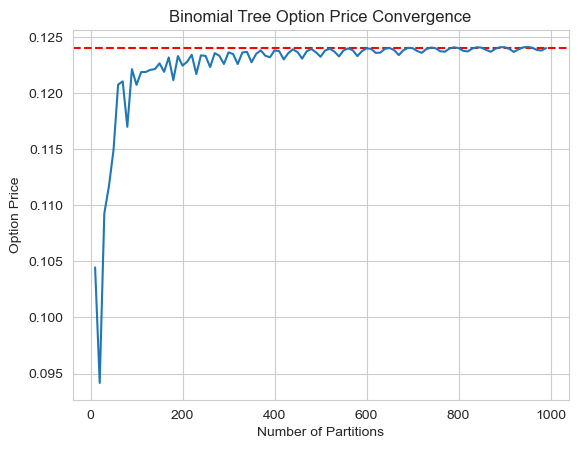
\includegraphics[scale=0.6]{./imgs/binomialtreeconvergence.png}
            \caption{Convergence of the binomial tree method with the number of partitions.}
      \end{figure}
\end{frame}
 
\begin{frame}{Question 4}
%       d) Use the binomial tree approach to estimate the price of a Jun 2024 American put option , where 𝑟 = 0.05 ,
% 𝑆0 = 𝑐𝑢𝑟𝑟𝑒𝑛𝑡 𝑝𝑟𝑖𝑐𝑒 , 𝐾 = 𝑆0 + $50
      \begin{itemize}
            \item Use the binomial tree approach to estimate the price of a Jun 2024 American put option.
            \item Given $r = 0.05$, $S_0 =  $current price, $K = S_0 + \$50$.
            \item We used the same formula as the European call option, but with the following changes:
            \begin{itemize}
                  \item $C_u = \max(K - S_u, 0)$, $C_d = \max(K - S_d, 0)$.
                  \item We used the early exercise condition to calculate the price of the American put option.
            \end{itemize}
      \end{itemize}

      \begin{tcolorbox}
            We find that the price of the American put option is $\boxed{47.78}$.
      \end{tcolorbox}
\end{frame}


\begin{frame}{Question 5}
%       # e) Use B-S formula to calculate the price of a Jun 2024 European call option , where 𝑟 = 0.05 , 𝑆0 =
% # 𝑐𝑢𝑟𝑟𝑒𝑛𝑡 𝑝𝑟𝑖𝑐𝑒 ,𝐾 = 𝑆0 + $50. Use the put-call parity relation to calculate the price of a corresponding put
% # option. Calculate the Delta, Gamma, Vega, rho of this option at the start of the option’s life.

      \begin{itemize}
            \item Given $r = 0.05$, $S_0 =  $current price, $K = S_0 + \$50$.
            \item We used the following formula to calculate the price of the European call option:
            \item $C = S_0 \times N(d_1) - K \times e^{-rT} \times N(d_2)$.
            \item Where $d_1 = \frac{\log(\frac{S_0}{K}) + (r + \frac{\sigma^2}{2})T}{\sigma \sqrt{T}}$, $d_2 = d_1 - \sigma \sqrt{T}$.
            \item We used the put-call parity relation to calculate the price of the corresponding put option.
      \end{itemize}

      \begin{tcolorbox}
            We find that the price of the European call option is $\boxed{0.1207}$.
            and the price of the corresponding put option is $\boxed{47.78}$. 
            This is essentially the same result as the Binomial Tree method.
      \end{tcolorbox}

\end{frame}

\begin{frame}{Question 5 $\Delta$}
      \begin{equation*}
            \frac{\partial C}{\partial S} = \frac{BS_{Call}(S+\Delta S, K, T,r,\sigma) - BS_{Call}(S, K, T,r,\sigma)}{\Delta S}
      \end{equation*}
      This equations essentially calculates the change in the price of the call option with respect to the change in the price of the underlying asset.
      \begin{tcolorbox}
            We find that the $\Delta$ of the European call option is $\boxed{0.0185}$.
      \end{tcolorbox}
\end{frame}

\begin{frame}{Question 5 $\Delta$ Continued}
      \begin{figure}
            \centering
            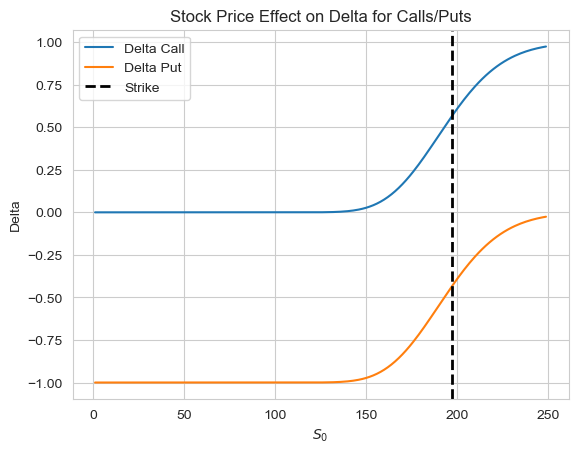
\includegraphics[scale=0.6]{./imgs/delta.png}
            \caption{Convergence of the $\Delta$ changing the price of $S_0$}
      \end{figure}

\end{frame}

\begin{frame}{Question 5 $\Delta$ Continued}
      \begin{figure}
            \centering
            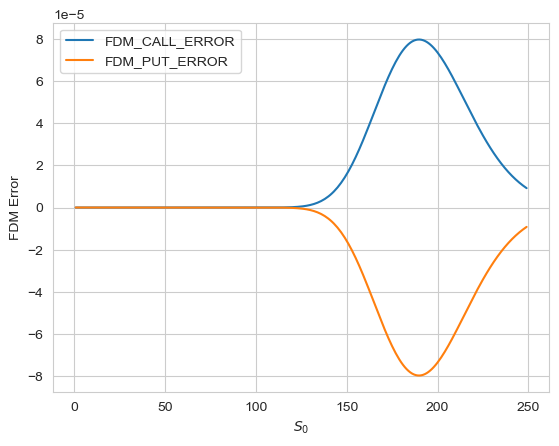
\includegraphics[scale=0.6]{./imgs/deltaerror.png}
            \caption{Error of the $\Delta$ changing the price of $S_0$}
      \end{figure}
\end{frame}

\begin{frame}{Question 5 $\Gamma$}
      \begin{equation*}
            \frac{\partial ^2{C}}{\partial S^2} =\frac{\partial ^2{P}}{\partial S^2} = \frac{N'(d_1)}{S\sigma\sqrt{T}}
      \end{equation*}

      If $\Delta$ is essentiall the ``speed'' of the option, then $\Gamma$ is the ``acceleration'' of the option.

      We use a finite difference method (FDM) to calculate the $\Gamma$ of the European call option.
      \tiny{
      \begin{equation*}
            \frac{\partial P}{\partial S} = \frac{BS_{Put}(S+\Delta S, K, T,r,\sigma) - 2BS_{Put}(S,K, T,r,\sigma) +BS_{Put}(S-\Delta S, K, T,r,\sigma)}{(\Delta S)^2}
      \end{equation*}
      }

      \normalsize

      \begin{tcolorbox}
            We find that the $\Gamma$ of the European call option is $\boxed{0.00184}$.
      \end{tcolorbox}
\end{frame}

\begin{frame}{Question 5 $\Gamma$ Continued}
      \begin{figure}
            \centering
            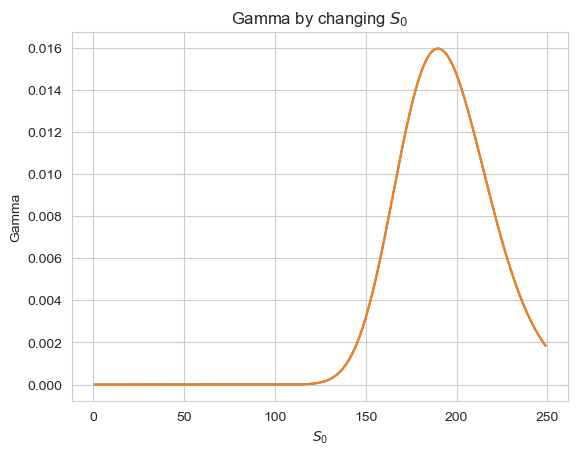
\includegraphics[scale=0.6]{./imgs/gamma.png}
            \caption{$\Gamma$ changing the price of $S_0$}
      \end{figure}

\end{frame}

\begin{frame}{Question 5 Vega}
      \begin{equation*}
            \frac{\partial {C}}{\partial \sigma} =\frac{\partial {P}}{\partial \sigma}=S\sqrt{T} N'(d1)
      \end{equation*}

      The Vega measures the sensitivity of the option price to changes in the volatility of the underlying asset.

      Vega Finite Difference Method (FDM) is used to calculate the Vega of the European call option.
      \tiny{
            \begin{equation*}
                  \frac{\partial C}{\partial \sigma} = \frac{BS_{Call}(S, K, T,r,\sigma) - BS_{Call}(S , K, T,r,\sigma -\Delta \sigma )}{\Delta \sigma}
            \end{equation*}
      }
      \normalsize
      \begin{tcolorbox}
            We find that the Vega of the European call option is $\boxed{3.26089}$.
      \end{tcolorbox}

\end{frame}

\begin{frame}{Question 5 Vega Continued}
      \begin{figure}
            \centering
            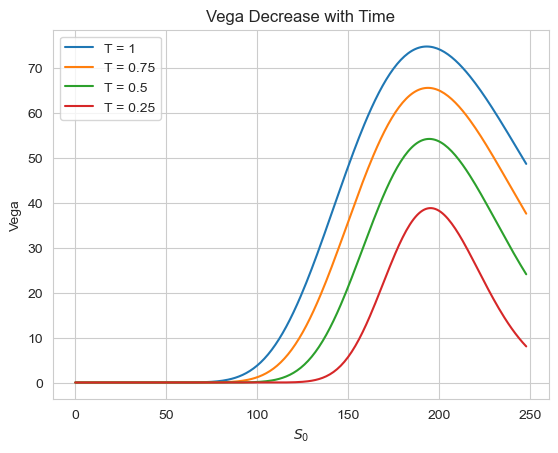
\includegraphics[scale=0.6]{./imgs/vega.png}
            \caption{Vega changing the value of $T$}
      \end{figure}

\end{frame}


\begin{frame}{Question 5 $\Theta$}
      \begin{equation*}
            \frac{\partial {C}}{\partial T} =\frac{\partial {P}}{\partial T}=-S_0N(d_1)\sigma\frac{1}{2\sqrt{T}} - rKe^{-rT}N(d_2)
      \end{equation*}

      The Theta measures the sensitivity of the option price to changes in time.

      Theta Finite Difference Method (FDM) is used to calculate the Theta of the European call option.
      \tiny{
            \begin{equation*}
                  \frac{\partial C}{\partial T} = \frac{BS_{Call}(S, K, T,r,\sigma) - BS_{Call}(S , K, T-\Delta T,r,\sigma)}{\Delta T}
            \end{equation*}
      }
      \normalsize
      \begin{tcolorbox}
            We find that the Theta of the European call option is $\boxed{-1.963}$.
      \end{tcolorbox}

\end{frame}

\begin{frame}{Question 5 $\Theta$ Continued}
      \begin{figure}
            \centering
            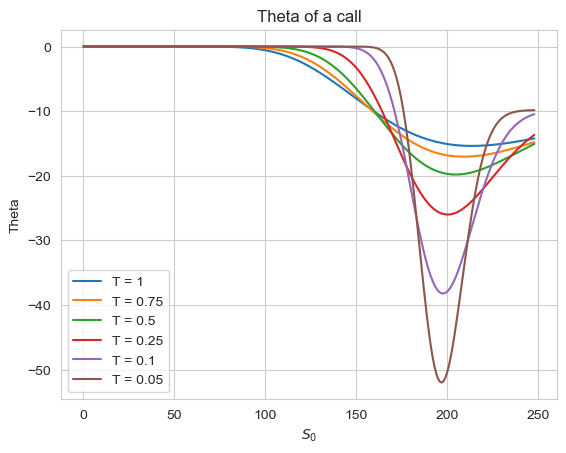
\includegraphics[scale=0.6]{./imgs/theta.png}
            \caption{Theta changing the value of $T$}
      \end{figure}

\end{frame}

\begin{frame}{Question 5 $\rho$}
      \begin{equation*}
            \frac{\partial {C}}{\partial r} =\frac{\partial {P}}{\partial r}=-KTe^{-rT}N(d_2)
      \end{equation*}

      The Rho measures the sensitivity of the option price to changes in the risk-free interest rate.

      Rho Finite Difference Method (FDM) is used to calculate the Rho of the European call option.
      \tiny{
            \begin{equation*}
                  \frac{\partial C}{\partial r} = \frac{BS_{Call}(S, K, T,r,\sigma) - BS_{Call}(S , K, T,r-\Delta r,\sigma)}{\Delta r}
            \end{equation*}
      }
      \normalsize
      \begin{tcolorbox}
            We find that the Rho of the European call option is $\boxed{0.620}$.
      \end{tcolorbox}
\end{frame}

\begin{frame}{Question 6}
%       Use a simple Monte Carlo method to estimate the price of a Jun 2024 European call option, where 𝑟 = 0.05
% 𝑆0 = 𝑐𝑢𝑟𝑟𝑒𝑛𝑡 𝑝𝑟𝑖𝑐𝑒 , 𝐾 = 𝑆0 + $50. Compare your answer with parts b) and e)

      \begin{itemize}
            \item Use a simple Monte Carlo method to estimate the price of a Jun 2024 European call option.
            \item Given $r = 0.05$, $S_0 =  $current price, $K = S_0 + \$50$.
            \item We used the following formula to calculate the price of the European call option:
            \begin{equation*}
                  C = e^{-rT} \left( \frac{1}{N} \sum_{i=1}^{N} \max(S_i - K, 0) \right)
            \end{equation*}
            \item Where $S_i = S_0 \times e^{(r - \frac{\sigma^2}{2})T + \sigma \sqrt{T} Z_i}$, $Z_i \sim N(0,1)$.
      \end{itemize}

\end{frame}

\begin{frame}{Question 6 Continued}
      \begin{tcolorbox}
            We find that the price of the European call option is not as accurate as the other methods. Most values are
            around $\$0$, which is different. We can take the mean of the values to get a better estimate, and we find that 
            the price of the European call option is $\boxed{1.3675}$, whereas the other methods gave us a price of $\$0.1207$.
      \end{tcolorbox}
\end{frame}

\begin{frame}{Question 6}
      % show 3 figures side by side (mc1.png, mcantithetic.png, mccontrol.png)
      \begin{figure}
            \centering
            \begin{subfigure}{0.4\textwidth}
                  \centering
                  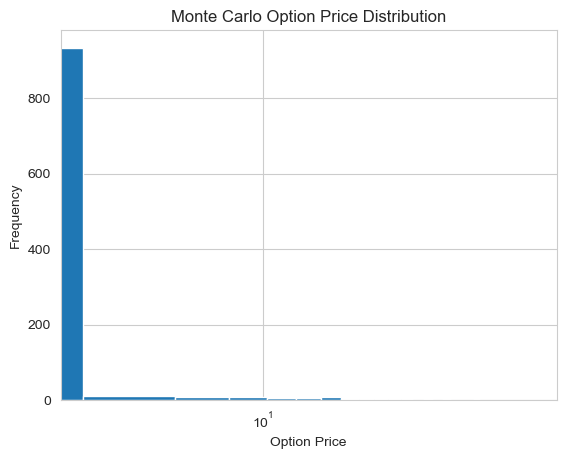
\includegraphics[scale=0.3]{./imgs/mc1.png}
                  \caption{Simple Monte Carlo}
            \end{subfigure}
            \begin{subfigure}{0.4\textwidth}
                  \centering
                  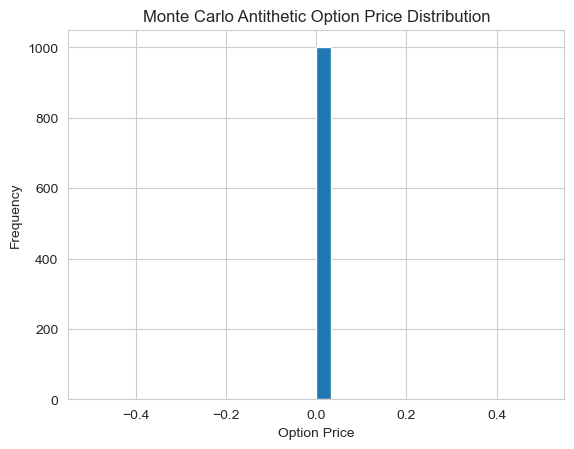
\includegraphics[scale=0.3]{./imgs/mcantithetic.png}
                  \caption{Antithetic Monte Carlo}
            \end{subfigure}
            \begin{subfigure}{0.4\textwidth}
                  \centering
                  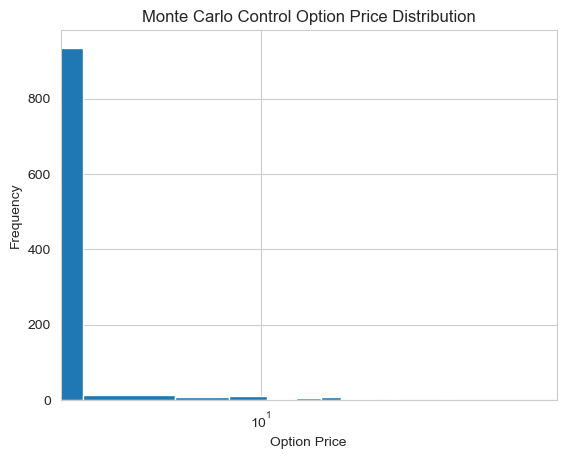
\includegraphics[scale=0.3]{./imgs/mccontrol.png}
                  \caption{Control Variate Monte Carlo}
            \end{subfigure}
            \caption{Comparison of the three Monte Carlo methods.}
      \end{figure}
      
\end{frame}

\begin{frame}{Question 7}

      \begin{itemize}
            \item Estimate the implied volatility for the problem in part e.
            \item We used the following formula to calculate the implied volatility:
            \begin{equation*}
                  \sigma = \text{optimize.newton}(f, 0.5)
            \end{equation*}
            \item Where $f(\sigma) = \text{black\_scholes}(S_0, K, T, r, \sigma, \text{option\_type}) - \text{price}$.
      \end{itemize}

      \begin{tcolorbox}
            We find that the implied volatility of the European call option is $\boxed{0.163}$,
            which is around half of the historical volatility.
      \end{tcolorbox}
\end{frame}

\End
\begin{frame}[plain,standout]
      \centering
      Questions?
\end{frame}

\end{document}

